
\documentclass[11pt, oneside]{article}   
\usepackage{pdfpages}
\usepackage{lscape}
\usepackage{geometry}                	
\geometry{letterpaper}                   		

\usepackage{graphicx}				
\usepackage{float}
\usepackage{multirow}
\usepackage{amssymb}

\renewcommand{\arraystretch}{1.5}
\usepackage{tabulary}
\usepackage{tabto}
\usepackage[newcommands]{ragged2e}

\usepackage{hyperref}
\hypersetup{
    colorlinks,
    citecolor=black,
    filecolor=black,
    linkcolor=blue,
    urlcolor=blue
}

\usepackage{titlesec}

\setcounter{secnumdepth}{4}

\titleformat{\paragraph}
{\normalfont\normalsize\bfseries}{\theparagraph}{1em}{}
\titlespacing*{\paragraph}
{0pt}{3.25ex plus 1ex minus .2ex}{1.5ex plus .2ex}

\usepackage{fancyhdr}
\usepackage{fancyhdr}
\fancyhead[L]{November 10, 2017}
\fancyhead[C]{SE 3XA3 Design Document}
\fancyhead[R]{Group 2: Genzter}
\pagestyle{fancy}

%SetFonts

%SetFonts


\title{SE 3XA3: Design Documentation Rev 0 \\ \textbf{Group 2}
}
\author{Bengezi, Mohamed - bengezim\\
		400021279
		\and
		Binu, Amit - binua\\
		400023175
		\and
		Samarasinghe, Sachin - samarya \\
		001430998}
\date{November 10, 2017}							


\begin{document}
\maketitle
\newpage

\tableofcontents\par
\listoftables
\listoffigures
\newpage


\section{Revision History}

\begin{table}[hp]
\caption{Revision History}
\begin{center}
\label{tab:}
\begin{tabular}{|c|c|c|c|}
\hline
\textbf{DATE} & \textbf{AUTHOR} & \textbf{DESCRIPTION} & \textbf{REVISION}\\
\hline
November 8, 2017 & Bengezi, Mohamed & Created Initial Document & 0\\
\hline
November 8, 2017 & Samarasinghe, Sachin & Initial Draft & 0\\
\hline
November 8, 2017 & Binu, Amit & Initial Draft & 0\\
\hline
\end{tabular}
\end{center}
\label{default}
\end{table}




\newpage
%---------------------------------------------------------------------
\section{Introduction}
\subsection{Brief Overview}
\tab This document outlines the Module Guide (MG), Module Interface Specification (MIS), and a Gantt chart detailing the schedule of implementation and testing. This project is a timetable generator, designed for McMaster University students, which allows students to select desired courses, and generates a set of schedules based on the input. 

\subsection{Design Overview}
\tab This document succeeds the SRS and precedes the MIS document. The SRS defines the functional and non-functional requirements of the system. The MG serves as a guide to users, and introduces new concepts, as well as prepares them for the MIS. The MIS breaks down what the system consists of, in a readable form. This means that the modules in the system are defined, and broken down. The SRS document's requirements are continually looked at and checked while creating the MG \& MIS, as well as used as a guideline when designing and implementing the modules. This document describes the Architectural Design and Detailed Design of the project. The goal of this document is to ensure the design and maintenance of the timetable generator by facilitating the successful interaction between modules in the program. The MG and MIS are created using the Separation of Concerns, Modularity, and Abstraction design principles. Separation of Concerns is when a problem is divided into smaller parts, or modules, and tackled individually. Modularity enables Separation of Concerns through Modular Decomposition, which is discussed in depth further in this document. Abstraction is used throughout in order to focus on the important aspects rather than minute details. 

\subsection{Document structure}
\tab This document is structured such that it contains an MG, which consists of likely/unlikely changes, module hierarchy, module decomposition trace-ability matrix between the SRS requirements and the modules. The document also contains MIS's for the various modules in the project, and lastly contains a schedule of the design, implementation, and testing tasks in the form of a Gantt chart. This structure is optimal because the Module Guide serves as an introduction, and equips the user with the knowledge necessary in order to fully understand the MIS. The MIS then allows users to see how the system is broken down into modules, and how those modules are broken down.

\newpage
\section{Anticipated \& Unlikely Changes}
\subsection{Anticipated Changes}
\begin{enumerate}
    \item AC1: Addition of a 'Generate again' button
    \item AC2: Drag and drop feature on output schedule
    \item AC3: Input UI
    \item AC4: Grammar/Syntax of JS/HTML/CSS 
\end{enumerate}

\subsection{Unlikely Changes}
\begin{enumerate}
    \item Input format (Course codes)
    \item Output (Will always be a schedule)
    \item Schedule Generation Algorithms
\end{enumerate}

%---------------------------------------------------------------------
\section{Module Hierarchy}

\begin{table}[H]
\begin{center}
\begin{tabular}{|c|c|c|}
\hline
\textbf{Level 1} & \textbf{Level 2}\\
\hline
Hardware-Hiding Module & N/A \\
\hline
Behaviour-Hiding Module & Input Parameters Module \\
& Scheduler Module \\
& Output Module \\
\hline
Software Decision Module & Course Module \\
\hline
\end{tabular}
\end{center}
\label{default}
\caption{Module Hierarchy}
\end{table}%


\newpage
\section{Connection of Requirements and Design}
\tab In the SRS document, there are functional requirements, such as getting user input, computing a valid schedule, and outputting in schedule format, and there are non-functional requirements, like simple usability, decent performance, and maintainability. Design decisions were made in order to satisfy these requirements. \\
\tab For gaining user input, as well as satisfy usability, a simple and elegant welcome page is designed. The page contains an input box that accepts course codes, and clear and concise instructions on the format of the course codes, as well as when to click the 'Add' and 'Generate' buttons. One the user has clicked the correct buttons, the input is then stored and used. In order to compute a valid schedule, a module dedicated to this is implemented, where it uses a graphing algorithm in order to create a schedule. A schedule output is achieved by creating an HTML table using an EJS module. Performance and Maintainability are ensured by following efficient programming procedures, as well as keeping clean and clear source code.

\newpage
\section{Module Decomposition}
\tab This section decomposes each module so that its secret, service, and implemented by information are known, and easy to understand. A secret is what the module is hiding, under the design principle of information hiding, by David Parnas. \cite{1} The service is what the module does. The implemented by section just describes how it is implemented

\subsection{Hardware Hiding Module} \\
\textbf{Secret:} How hardware differences are hidden from software \\
\textbf{Service:} Acts as an interface between the hardware and software \\
\textbf{Implemented By:} Operating System \\

\subsection{Behaviour Hiding Module}
\textbf{Secret:} Behaviours of System \\
\textbf{Service:} Implementing the various expected behaviours of the system \\
\textbf{Implemented By:} N/A \\

\subsubsection{Input Parameters Module}
\textbf{Secret:} Input \\
\textbf{Service:} Allowing users to enter desired information, in this case course codes \\
\textbf{Implemented By:}  Main.js, checkCourse.js \\

\subsubsection{Scheduler Module}
\textbf{Secret:} Computation \\
\textbf{Service:} Generates a schedule with selected input \\
\textbf{Implemented By:} scheduler.js \\

\subsubsection{Output Module}
\textbf{Secret:} Output \\
\textbf{Service:} Creates a visual table with time-slots of selected courses \\
\textbf{Implemented By:} schedule.ejs \\

\subsection{Software Decision Module}
\textbf{Secret:} Generic Modules and Data Structures\\
\textbf{Service:} House generic modules, and data structures that can be used by other applications \\
\textbf{Implemented By:} N/A \\

\subsection{Course Module}
\textbf{Secret:} Course Data Structure \\
\textbf{Service:} Provide a data structure for a course object \\
\textbf{Implemented By:} Course.js \\


\newpage



\section{Traceability Matrix}
The requirements used in the following matrix are from the SRS Document. The labels, such as 3.1, refer to the section in the SRS document.

\begin{table}[H]
\begin{center}
\begin{tabulary}{1\textwidth}{|c|c|}
\hline
Module & Label \\
\hline
Hardware Hiding Module & M1\\
\hline
Input Parameters Module & M2\\
\hline
Scheduler Module & M3\\
\hline
Output Module & M4\\
\hline
Course Module & M5\\
\hline
\end{tabulary}
\end{center}
\label{default}
\caption{Module Labels}
\end{table}

\subsection{Requirements Traceability Matrix}
\begin{table}[H]
\begin{center}
\begin{tabulary}{1\textwidth}{|c|c|}
\hline
Requirements & Modules \\
\hline
3.1 & M2, M5\\
\hline
3.2 & M3, M5\\
\hline
3.3 & M3, M4, M5\\
\hline
4.1.1 & M2, M4\\
\hline
4.1.2 & M1, M2, M3, M4, M5, M6\\
\hline
4.1.4 & M2, M3, M4, M5, M6\\
\hline
\end{tabulary}
\end{center}
\label{default}
\caption{Requirements Traceability Matrix}
\end{table}


\subsection{Anticipated Changes Traceability Matrix}
\begin{table}[H]
\begin{center}
\begin{tabulary}{1\textwidth}{|c|c|}
\hline
Anticipated Changes & Modules \\
\hline
AC1 & M3, M4\\
\hline
AC2 & M3, M4\\
\hline
AC3 & M2\\
\hline
AC4 & M2, M3, M4, M5\\
\hline
\end{tabulary}
\end{center}
\label{default}
\caption{Anticipated Changes Traceability Matrix}
\end{table}


\newpage
\section{Uses Hierarchy}

\begin{figure}[h]
    \centering
    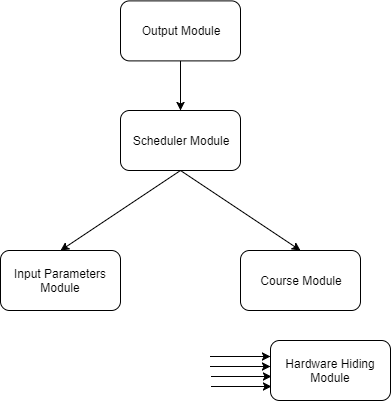
\includegraphics[height=127mm]{Attachments/UsesRelation.png}
    \caption{Uses Relation}
    \label{fig:my_label}
\end{figure}


\newpage

\section{MIS's of app.js}
\subsection*{Template Module}
course
\subsection* {Uses}
N/A
\subsection* {Syntax}
\subsubsection* {Exported Types}
app = ?
\subsubsection* {Exported Access Programs}
\begin{tabular}{| l | l | l | l |}
\hline
\textbf{Routine name} & \textbf{In} & \textbf{Out} & \textbf{Exceptions}\\
\hline
startProgram & - & - & UrlNotFoundException \\
\hline

\end{tabular}
\subsection* {Semantics}
\subsubsection* {State Variables}
$courseIds$:= Course ids of all the courses offered in McMaster University \\ \\
$allCourses$:= Matrix of all the information about all the courses offered in McMaster University
\subsubsection*{Environment Variables}
Screen: Display Output Device \\

\subsubsection* {State Invariant}
none
\subsubsection* {Assumptions}
It is assumed that the url used to fetch the data is always online. 
\subsubsection* {Access Routine Semantics}
startProgram():
\begin{itemize}
\item transition: Updates the $courseIds$ to have the course ids of all courses and $allCourses$ to have all the information (such as Prof name, room, courseId etc) of all the courses.
\item output: $none$
\item exception:
 none
\end{itemize}




\newpage

\section{MIS's of checkCourse.js}
\subsection*{Template Module}
course
\subsection* {Uses}
app.js
\subsection* {Syntax}
\subsubsection* {Exported Types}
router = ?
\subsubsection* {Exported Access Programs}
\begin{tabular}{| l | l | l | l |}
\hline
\textbf{Routine name} & \textbf{In} & \textbf{Out} & \textbf{Exceptions}\\
\hline
submit & Request,Response,Next & string & -\\
\hline
check &  Array of strings & Boolean& -\\
\hline
\end{tabular}
\subsection* {Semantics}
\subsubsection* {State Variables}
None
\subsubsection*{Environment Variables}
Screen: Display Output Device \\
Keyboard: Input Device \\

\subsubsection* {State Invariant}
none
\subsubsection* {Assumptions}
None
\subsubsection* {Access Routine Semantics}
submit($req, res, next$):
\begin{itemize}
\item transition: none
\item output: Outputs a string message to the user's browser if there were any problems with user's input, otherwise it will return null. 
\item exception:
 none
\end{itemize}
\\
\noIndent
check($selectedCourses$):
\begin{itemize}
\item transition: none
\item output: Outputs a Boolean value, true if there were no problems with user's input, and false if there was. 
\item exception:
 none
\end{itemize}


\newpage

\section{MIS's of index.js}
\subsection*{Template Module}
course
\subsection* {Uses}
app.js
checkCourse.js
scheduler.js
\subsection* {Syntax}
\subsubsection* {Exported Types}
router = ?
\subsubsection* {Exported Access Programs}
\begin{tabular}{| l | l | l | l |}
\hline
\textbf{Routine name} & \textbf{In} & \textbf{Out} & \textbf{Exceptions}\\
\hline
welcomePage & Request,Response,Next & EJS file & -\\
\hline
giveLink &  Request,Response,Next & EJS file & -\\
\hline

\end{tabular}
\subsection* {Semantics}
\subsubsection* {State Variables}
None
\subsubsection*{Environment Variables}
Screen: Display Output Device \\
Keyboard: Input Device \\

\subsubsection* {State Invariant}
none
\subsubsection* {Assumptions}
None
\subsubsection* {Access Routine Semantics}
welcomePage($req, res, next$):
\begin{itemize}
\item transition: none
\item output: Sends an ejs template to the user's browser
\item exception:
 none
\end{itemize}
\\
\noIndent
giveLink($req, res, next$):
\begin{itemize}
\item transition: none
\item output: Sends an ejs template to the user's browser
\item exception:
 none
\end{itemize}
\newpage

\section{MIS's of scheduler.js}
\subsection*{Template Module}
course
\subsection* {Uses}
Course.js \\
checkCourse.js \\
app.js \\

\subsection* {Syntax}
\subsubsection* {Exported Types}
router = ? \\
reset  = ? \\

\subsubsection* {Exported Access Programs}
\begin{tabular}{| l | l | l | l |}
\hline
\textbf{Routine name} & \textbf{In} & \textbf{Out} & \textbf{Exceptions}\\
\hline
start & req, res,next & EJS file & -\\
\hline
getSchedule & req, res, next & - & - \\
\hline
algorithm & - & Boolean & - \\
\hline
permutation & int & int & - \\
\hline
updateSemester & List & List & - \\
\hline
dobothSemester & List, List, List & List & - \\
\hline
MadeBefore & List, List & Boolean & - \\
\hline
Conflicts & int, int, int & Boolean & - \\
\hline
prioritize & List & List & - \\
\hline
doSemester & List & Boolean & - \\
\hline
makeGraph & - & Boolean & - \\
\hline
getConnectedComponent & Graph & List & - \\
\hline
reserveTime & int, int, int & - & - \\
\hline
avoidConflicts & int, int, int, int & - & - \\
\hline
hasConflict & int, int, int, int & Boolean & - \\
\hline
hasPathConflict & int, int, int, int & Boolean & - \\
\hline
BreadthFirstPaths & Graph, int & - & - \\
\hline
bfs & Graph , int & - & - \\
\hline
hasPathTo & int & Boolean & - \\
\hline
putInaDay & int, String & - & - \\
\hline



\end{tabular}
\subsection* {Semantics}
\subsubsection* {State Variables}
$graph:$ Graph - a graph where each node represents a course and an edge represents a conflict-less relationship between courses  \\ \\
$ dataset:$ List of strings - array that represents the data-set  \\ \\
$ allCourses:$ List of strings - List of  course codes all courses available in McMaster University \\ \\
$finalCourses:$List of strings - List of course codes the user added \\ \\
$bothSemesters:$ List of strings - List of course codes of courses that are offered in both Semesters \\ \\

$semester1:$ List of strings - List of course codes of the courses that are available only in semester 1 \\ \\

$semester2:$ List of strings - List of course codes of the courses that are available only in semester 2 \\ \\

$fixedCores:$ List of strings - List of course codes of courses with one core(lab,lecture,tutorial). e.g) "SFWRENG 2XA3 C01" \\ \\ 

$flexCores:$ List of strings - List of course codes of courses with more than one core(lab,lecture,tutorial). e.g) "SFWRENG 2XA3 L01 , SFWRENG 2XA3 L02" 

$finalSemester1:$ List of timeObjects - List of timeObjects that for final semester 1 schedule \\ \\ 

$finalSemester2:$ List of timeObjects - List of timeObjects that for final semester 2 schedule \\ \\ 

$ day1:$ List Course Objects - List of course objects of courses that are on Monday of the final schedule. \\ \\ 

$ day2:$ List of Course Objects - List of course objects of courses that are on Tuesday of the final schedule. \\ \\ 

$ day3:$ List of Course Objects - List of course objects of courses that are on Wednesday of the final schedule. \\ \\ 

$ day4:$ List of Course Objects - List of course objects of courses that are on Thursday of the final schedule. \\ \\ 

$ day5:$ List of Course Objects - List of course objects of courses that are on Friday of the final schedule. \\ \\ 

$ day6:$ List of Course Objects - List of course objects of courses that are on Saturday of the final schedule. \\ \\ 

$ times: $ 2D Matrix of double - The values in this array represents the times reserved by courses. This is used to check for conflicts between courses. \\ \\

$ success:$ Boolean - The value of this variable represents the success of the program. True means a schedule was generated, false means there was an error.\\ \\

$ schedule:$ List of strings - List of course objects of fixed cores that are in the final semester 1 schedule.\\ \\

$ schedule2: $ List of strings - List of course objects of fixed cores that are in the final semester 2 schedule.\\ \\

$ madeArrays:$ 2D Matrix of integers - This array keeps track of different versions of arrays that were made by shuffling its elements. \\ \\

$ conflictCourses:$ List of strings - List of course codes of courses that conflicts with each other.\\ \\

$ conflictAvoider:$ List of double - Each element in this array represents the times between and including the starting and ending time of a lecture/lab/tutorial.\\ \\

$ allTimeObjects:$ List of timeObjects - This array contains the time objects of all cores(lab,lecture, tutorial) of all the courses the user selected.\\ \\

$ marked: $ List of Boolean - This array is used to get the BreadFirstPath in a graph\\ \\
$ edgeTo:$ List of real - This array is used to get the BreadFirstPath in a graph\\ \\
$ distTo:$ List of real - This array is used to get the BreadFirstPath in a graph\\ \\
$ q:$List of real - This array is used to get the BreadFirstPath in a graph\\ \\

\subsubsection*{Environment Variables}
Screen: Display Output Device \\

\subsubsection* {State Invariant}
none
\subsubsection* {Assumptions}
None
\subsubsection* {Access Routine Semantics}
start($req, res,next$):
\begin{itemize}
\item This routine starts the calculations for generating a schedule by calling other routines and initializing some global variables.
\item transition: $schedule,
    times,
    day1,
    day2,
    day3,
    day4,
    day5,
    day6, \newline
    semester1 ,
    semester2 ,
    bothSemesters ,
    fixedCores,
    flexCores,
    finalSemester1,
    finalSemester2 $ := [\hspace{0.2cm}],[\hspace{0.2cm}],[\hspace{0.2cm}],[\hspace{0.2cm}],[\hspace{0.2cm}],[\hspace{0.2cm}],[\hspace{0.2cm}],[\hspace{0.2cm}],[\hspace{0.2cm}],[\hspace{0.2cm}],[\hspace{0.2cm}],[\hspace{0.2cm}],[\hspace{0.2cm}],[\hspace{0.2cm}],[\hspace{0.2cm}]
\item output: $EJS file$
 \item exception: none
\end{itemize}


\noindent
getschedule(req,res,next)
\begin{itemize}
\item This routine sends the generated schedule to the user's browser.
\item transition: none
\item output: $EJS file$
 \item exception: none
\end{itemize}

\noindent
algorithm()
\begin{itemize}
\item This routine finds the courses that are offered only in semester1, only in semester 2 and in both semesters, and then they are put in proper arrays.
\item transition: $semester1, semester2, bothSemesters,sucess $ := $\{$string, string ...$\}$,$\{$string, string ...$\}$,$\{$string, string ...$\}$, boolean
\item output: $EJS file$
 \item exception: none
\end{itemize}

\noindent
permutation(number)
\begin{itemize}
\item This routine finds the total permutation by calculating the factorial of a given number.
\item transition: none
\item output: $ int $ - Outputs an integer that is the factorial of the input $number$
 \item exception: none
\end{itemize}

\noindent
updateSemester(semester)
\begin{itemize}
\item This routine creates a duplicate of an array and outputs it.
\item transition: none
\item output: - Outputs a duplicate of the given array ( $semester$ )in the input.
 \item exception: none
\end{itemize}

\noindent
dobothSemester(bothSemesters,semester1,semester2)
\begin{itemize}
\item This routine re-orders the courses in $bothSemester$ and tries to put them in $semester1$ and $semester 2$.Then, it calls the routine $doSemester(semester)$ twice, one time with $semester1$ and the other time with $semester2$. 
If a working schedule is found, it will return an array of bothSemesters that are arranged in a specific way which will generate a schedule, when they are put in semester1 and semester2.
\item transition: none
\item output: - Outputs an empty array if there is no way to make a schedule. If it is possible to make a schedule, it will output an array with courses in bothSemester arranged in a specific way.
 \item exception: none
\end{itemize}

\noindent
MadeBefore(madeArrays,arr)
\begin{itemize}
\item This routine checks if $madeArrays$ have the array $arr$.
\item transition: none
\item output: - Outputs a boolean value, true if the $arr$ is in $madeArrays$ and false if it is not.
 \item exception: none
\end{itemize}

\noindent
Conflicts(startTime,endTime,day)
\begin{itemize}
\item This routine checks if the array , in the state variable $times$ ,  at index d have any values between and including, startTime \& endTime. If it does, it return true and if it doesn't then it returns false.
\item transition: none
\item output: - Outputs a Boolean value, true if any values between and including starting \& endTime are in the array in $times$ at index $day$.
 \item exception: none
\end{itemize}

\noindent
prioritize(semester)
\begin{itemize}
\item This routine reorders the array $semester$ based upon how many lectures,tutorials and labs a course has.If a course in $semester$ has the most number of lectures,tutorials and labs, then it will be placed in the beginning of the array.
\item transition: none
\item output: - Outputs a new array that has the courses in $semester$ but in a different order.
 \item exception: none
\end{itemize}
\noindent


doSemester(semester)
\begin{itemize}
\item This routine updates the state variables $fixedCores$ and $flexCores$ by putting the courses that offer only one lecture or one tutorial or one lab in $fixedCores$. It puts the cores($Example\hspace{0.1cm} of \hspace{0.1cm}core: PHYSICS \hspace{0.1cm}1e03\hspace{0.1cm} c01,\hspace{0.1cm} chem\hspace{0.1cm}2e03\hspace{0.1cm} T01 $) that offer more than one lecture or more than one tutorial or more than one lab in $flexCores$. It also tries to find if there is any conflict between courses in $fixedCores$
\item transition: $fixedCores,flexCores :=$ \{string,string...\},\{string,string...\}
\item output: - Outputs a Boolean, true if there were no conflicts between cores in $fixedCores$ and false if there is.
 \item exception: none
\end{itemize}

\noindent
makeGraph()
\begin{itemize}
\item This routine makes a graph where each node is a course and each edge represents a conflict-less relationship between two courses.
\item transition: none
\item output: - Outputs a Boolean, true if it is possible to make a graph with cores from all courses.
 \item exception: none
\end{itemize}

\noindent
getConnectedComponent(graph)
\begin{itemize}
\item This routine finds all the nodes that are connected to at least one other node. The cores that are not connected are ignored.
\item transition: none
\item output: - Outputs an array with all the cores that are connected to at least one other core.
 \item exception: none
\end{itemize}

\noindent
reserveTime(startTime,endTime,day)
\begin{itemize}
\item This routine puts all the values between(and including) $startTime$ and $endTime$ in an array that is at the index $day$ of the state variable $times$
\item transition: $times:=$ \{\{double,double,double\},\{double,double,double\},\{double,double,double\},\newline\{double,double,double\},\{double,double,double\},\{double,double,double\},\{double,double,double\}\}
\item output: - none
 \item exception: none
\end{itemize}

\noindent
avoidConflicts(startTime,endTime,day,courseIndex)
\begin{itemize}
\item transition: This routine puts all the times between (and including) $startTime$ and $endTime$ at $conflictAvoider[courseIndex][day]$.
\item output: none
 \item exception: none
\end{itemize}

\noindent
hasConflict(startTime,endTime,day,courseId)
\begin{itemize}

\item transition: none
\item output: Ouputs a Boolean, true if the state variable $conflictAvoider$ has any values between (and including) $startTime$ and $endTime$ at $conflictAvoider[courseIndex][day], and false if it doesn't.
 \item exception: none
\end{itemize}
\\

\noindent
hasPathConflict(coreId,day, start,end)
\begin{itemize}
\item transition: none
\item output: Outputs a Boolean, true if there is a conflict between any courses that are in path between node 0 and the node at coreId and false if it is not.
 \item exception: none
\end{itemize}

\noindent
BreadthFirstPaths(graph, start)
\begin{itemize}
\item transition: Updates the values of state variables $marked$, $edgeTo$, $distTO$ based upon the graph algorithm. This routine is a part of the graph algorithm.
\item output: none
 \item exception: none
\end{itemize}

\noindent
bfs(G, s)
\begin{itemize}
\item transition: Updates the values of state variables $marked$, $edgeTo$, $distTO$ based upon the graph algorithm. This routine is a part of the graph algorithm.
\item output: none
 \item exception: none
\end{itemize}

\noindent
hasPathTo(v)
\begin{itemize}
\item transition: none
\item output: Outputs a boolean, true if there is a path to specified node from node 0 and false if there is no path. This routine is a part of the graph algorithm.
\item exception: none
\end{itemize}

\noindent
putInaDay(courseDay, course)
\begin{itemize}
\item transition: Depending on the value of $courseDay$, it will update either the state variable day1 or day2 or day3 or day4 or day5 or day6 , by pushing the value of course into one of the arrays that was mentioned before.
\item output: none
\item exception: none
\end{itemize}


\newpage
%---------------------------------------------------------------------
\section{Schedule}
\includepdf[pages={5},landscape=true]{Attachments/Schedule.pdf}
%---------------------------------------------------------------------


\newpage
\begin{thebibliography}{9}
\bibitem{1} 
On the Criteria To Be Used in Decomposing Systems into Modules 
\textit{D.L. Parnas}
\url{https://www.cs.umd.edu/class/spring2003/cmsc838p/Design/criteria.pdf}


 
\end{thebibliography}
\end{document}  